%% =============================================================
%%  L'interprétation — mouvements, nuances, articulations, caractère
%%  Guide de référence, composé en LaTeX, gravures LilyPond
%% =============================================================
%%
%%  Les tableaux (gravures/interpretation-*.tex), les figures
%%  (gravures/ip-*.cropped.pdf), les énoncés et les réponses des
%%  exercices et le fichier interpretation.musicxml sont produits par
%%  outils/generer_interpretation.py. Voir le colophon en dernière page.
%%
\documentclass[a4paper,11pt]{article}

\usepackage[top=2.2cm,bottom=2.4cm,left=2.2cm,right=2.2cm]{geometry}
\usepackage[T1]{fontenc}
\usepackage[utf8]{inputenc}
\usepackage[french]{babel}
\usepackage{lmodern}
\usepackage{xcolor}
\usepackage{graphicx}
\usepackage{titlesec}
\usepackage{fancyhdr}
\usepackage{mdframed}
\usepackage{enumitem}
\usepackage{booktabs}
\usepackage{hyperref}

\graphicspath{{gravures/}}

% ---- Couleurs, reprises du document des accords de guitare ---------
\definecolor{navy}{RGB}{18,50,105}
\definecolor{lightnavy}{RGB}{235,241,255}
\definecolor{mygray}{RGB}{110,110,110}

\hypersetup{colorlinks=true, linkcolor=navy, urlcolor=navy,
  pdftitle={L'interprétation — mouvements, nuances, articulations, caractère},
  pdfauthor={Fabian Bastin}}

% ---- En-tête et pied -----------------------------------------------
\pagestyle{fancy}
\fancyhf{}
\renewcommand{\headrulewidth}{0.4pt}
\renewcommand{\footrulewidth}{0.4pt}
\fancyhead[L]{\small\bfseries\textcolor{navy}{L'interprétation}}
\fancyhead[R]{\small\textcolor{mygray}{\thepage}}
\fancyfoot[C]{\small\textcolor{mygray}{Mouvements, nuances, articulations, caractère}}

% ---- Titres de section ---------------------------------------------
\newcommand{\navysect}[1]{%
  \colorbox{navy}{%
    \parbox[c][17pt]{\dimexpr\linewidth-2\fboxsep\relax}{%
      \color{white}\hspace{6pt}\bfseries\normalsize #1}}%
}
\titleformat{\section}[block]{\normalfont}{}{0pt}{\navysect}
\titlespacing*{\section}{0pt}{16pt}{10pt}

% ---- Encadré de remarque -------------------------------------------
\newmdenv[linecolor=navy, linewidth=0.5pt, backgroundcolor=lightnavy,
  innertopmargin=6pt, innerbottommargin=6pt,
  innerleftmargin=8pt, innerrightmargin=8pt,
  skipabove=8pt, skipbelow=8pt]{remarque}

% ---- Figure gravée ---------------------------------------------------
% Figure gravée, à la largeur donnée (part de la ligne), avec sa légende.
% Le tout tient dans une minipage : figure et légende ne sont jamais
% séparées par un saut de page.
\newcommand{\gravure}[3]{%
  \par\medskip\noindent
  \begin{minipage}{\linewidth}
    \centering
    \includegraphics[width=#2\linewidth]{#1.cropped.pdf}\\[4pt]
    {\small\itshape\color{mygray} #3}
  \end{minipage}\par\medskip
}

% Un tableau produit par le générateur, centré.
\newcommand{\tableau}[1]{%
  \par\medskip
  {\centering\small\input{gravures/interpretation-#1.tex}\par}
  \medskip
}

% Le segno et la coda, gravés, dans le texte.
\newcommand{\segno}{\raisebox{-0.2ex}{
\includegraphics[height=2.2ex]{ip-segno.cropped.pdf}}}
\newcommand{\coda}{\raisebox{-0.2ex}{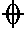
\includegraphics[height=2.2ex]{ip-coda.cropped.pdf}}}

% Une nuance : lettres italiques grasses.
\newcommand{\nuance}[1]{\textbf{\emph{#1}}}

\setlist{itemsep=2pt, topsep=4pt, parsep=0pt}

\begin{document}

% =====================================================================
\begin{titlepage}
\centering
\vspace*{3cm}
{\Huge\bfseries\color{navy} L'interprétation\par}
\vspace{0.6cm}
{\LARGE\color{navy} Mouvements, nuances, articulations, caractère\par}
\vspace{1.4cm}
{\large Ce que la partition dit en plus des notes\par}
\vspace{2.5cm}
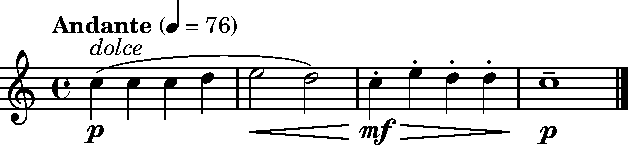
\includegraphics[width=0.75\linewidth]{ip-phrase.cropped.pdf}
\vfill
{\small\color{mygray}
Gravures LilyPond, composition \LaTeX.\\
Fichier MusicXML joint.\par}
\vspace{1cm}
\end{titlepage}

\tableofcontents
\newpage

% =====================================================================
\section{Avant-propos}

Les notes disent quoi jouer ; d'autres indications disent comment. Le
\textbf{mouvement} règle l'allure, les \textbf{nuances} l'intensité, les
\textbf{articulations} la façon d'attaquer les notes et de les enchaîner, les
termes de \textbf{caractère} l'esprit du jeu. La plupart sont des mots
italiens : l'usage s'en est fixé aux XVII\textsuperscript{e} et
XVIII\textsuperscript{e} siècles, quand la musique italienne servait de modèle
à toute l'Europe, et ils sont restés en usage partout.

Au programme de matières théoriques de l'École de musique Vincent-d'Indy, ces
notions relèvent des niveaux 4 et 5. Elles supposent connues les valeurs et la
mesure, dont traitent \href{https://www.slashbin.net/musique/theorie/valeurs.pdf}{\emph{Les valeurs}} et \href{https://www.slashbin.net/musique/theorie/mesure.pdf}{\emph{La mesure}} : un mouvement se
compte en temps par minute, et une articulation agit sur la durée réelle d'une
valeur écrite.

\gravure{ip-phrase}{0.75}{Les quatre familles sur une même phrase : en tête, le
mouvement (\emph{Andante}) et le caractère (\emph{dolce}) ; sous la portée, les
nuances ; sur les notes, les articulations --- une liaison, des points de
\emph{staccato}, un trait de \emph{tenuto}.}

\begin{remarque}
\textbf{Conventions.} Les termes italiens sont en italique, suivis de leur sens
littéral. Un mouvement se donne en pulsations par minute : «~noire = 80~»
demande quatre-vingts noires à la minute. Les exemples sont en clé de sol et en
do majeur ; la plupart reprennent une même phrase, \emph{Au clair de la lune},
pour qu'on entende ce que change chaque indication.
\end{remarque}

Le fichier MusicXML joint fait entendre ces exemples ; la
section~\ref{sec:musicxml} le présente.

% =====================================================================
\section{Les mouvements}
\label{sec:mouvements}

\textbf{L'allure des temps.} Le mouvement est la vitesse de la pulsation,
c'est-à-dire des temps de la mesure. Il s'écrit en tête du morceau, au-dessus
de la première portée, d'un mot italien souvent suivi d'une indication
métronomique : «~\emph{Allegro} (noire = 132)~» demande un mouvement vif, à
cent trente-deux noires par minute.

\textbf{Du plus lent au plus vif.} Le tableau range les mouvements usuels. Leur
sens littéral rappelle que ces mots disaient d'abord une manière d'être :
\emph{allegro} veut dire gai, \emph{andante} «~allant~», du verbe \emph{andare},
aller, et \emph{adagio} vient de \emph{ad agio}, à l'aise.

\tableau{mouvements}

\begin{remarque}
\textbf{Des fourchettes indicatives.} Les nombres ne donnent qu'un ordre de
grandeur. Ils varient d'un tableau à l'autre, et les métronomes mécaniques
impriment souvent sur leur tige leurs propres bandes, semblables à celles-ci.
Parmi les plus lents, l'ordre lui-même varie selon les auteurs et les époques :
\emph{grave}, \emph{largo}, \emph{lento} et \emph{adagio} échangent parfois
leur place. Un même mot, enfin, ne donne pas le même tempo dans toutes les
musiques : il dit autant un caractère qu'une vitesse.
\end{remarque}

\textbf{Diminutifs et superlatifs.} Le suffixe \emph{-etto} atténue :
\emph{larghetto} est un peu moins lent que \emph{largo}, \emph{allegretto} un
peu moins vif qu'\emph{allegro}. Le suffixe \emph{-issimo} renforce :
\emph{prestissimo} va plus vite que \emph{presto}. Le sens
d'\emph{andantino}, diminutif d'\emph{andante}, a longtemps hésité : un peu
plus lent qu'\emph{andante} pour les uns, un peu plus allant pour les autres ;
ce second sens l'emporte aujourd'hui.

\textbf{Au pas d'une danse.} Un mouvement se nomme parfois d'après une danse :
\emph{Tempo di minuetto}, au mouvement d'un menuet ; \emph{Tempo di valse},
d'une valse.

\textbf{Le métronome.} Johann Nepomuk Maelzel fait breveter le métronome en
1815. Beethoven, l'un des premiers à s'en servir, publie en 1817 les
indications métronomiques de ses huit premières symphonies. Les lettres
«~M.M.~» qui précèdent parfois le nombre signifient «~métronome de Maelzel~».

\textbf{Changer de mouvement.} D'autres termes modifient le mouvement en cours
de route.

\tableau{changements}

Les changements progressifs --- \emph{accelerando}, \emph{rallentando},
\emph{ritardando} --- durent jusqu'à l'indication suivante ; un trait pointillé
après l'abréviation en montre souvent l'étendue. \emph{A tempo} ramène au
mouvement d'avant le changement, \emph{tempo primo} à celui du début.
\emph{Ritenuto} ralentit d'un coup, là où \emph{ritardando} ralentit peu à
peu ; l'abréviation \emph{rit.} sert parfois aux deux, et le contexte tranche.
\emph{L'istesso tempo} garde la pulsation quand la mesure change : la noire d'un
2/4 devient, par exemple, la noire pointée d'un 6/8. \emph{Ad libitum} et
\emph{a piacere} laissent le mouvement à l'interprète, le temps d'un passage ;
sur une partie d'instrument, \emph{ad libitum} dit aussi qu'on peut s'en passer.

\gravure{ip-tempo}{1}{Un \emph{Allegro} ralenti à partir de la troisième
mesure : le trait qui suit \emph{rit.} dure autant que le ralentissement, et
\emph{a tempo} rend le mouvement du début.}

\textbf{Le temps dérobé.} Avec le \emph{tempo rubato}, l'interprète presse ici
et retient là, pour faire chanter la phrase, sans que la pulsation d'ensemble
se perde. On l'associe surtout à la musique romantique, à Chopin en
particulier ; il s'écrit rarement, il se pratique.

\textbf{Le point d'orgue.} Le point d'orgue suspend la mesure sur une note ou
un silence ; il relève des valeurs, et \emph{Les valeurs} en traitent.

% =====================================================================
\section{Les nuances}
\label{sec:nuances}

\textbf{Doux et fort.} Deux mots italiens suffisent : \emph{piano}, doux, et
\emph{forte}, fort. \emph{Mezzo}, à moitié, les modère ; le superlatif
\emph{-issimo} les pousse plus loin. Ils s'abrègent en lettres italiques grasses
placées sous la portée --- au piano, entre les deux portées --- et valent
jusqu'à la nuance suivante.

\tableau{nuances}

\gravure{ip-nuances}{0.8}{Les six nuances usuelles, du plus doux au plus fort.}

\textbf{Des degrés, non des mesures.} Une nuance ne se mesure pas : elle situe
un passage par rapport aux autres, selon l'instrument, la salle et le style. Les
extrêmes vont plus loin, \nuance{ppp} ou \nuance{fff}, et Tchaïkovski écrit
même \nuance{pppppp} dans le premier mouvement de sa \emph{Symphonie
pathétique}. Des mots disent aussi la nuance par la voix : \emph{sotto voce}, à
voix basse, et \emph{mezza voce}, à mi-voix.

\textbf{Changer de nuance.} Le \emph{crescendo} et le \emph{decrescendo}
s'écrivent en toutes lettres, abrégés et suivis d'un trait pointillé, ou par
des \emph{soufflets}, deux traits qui s'ouvrent ou se referment sur la durée du
changement. \emph{Diminuendo} et \emph{decrescendo} sont synonymes. D'autres
changements sont soudains : \emph{subito} s'ajoute à une nuance pour qu'elle
tombe d'un coup, le \emph{sforzando} appuie une seule note, et le
\emph{forte-piano} attaque fort pour retomber aussitôt dans le doux. Le
\emph{rinforzando} renforce de même quelques notes, ou une courte phrase.
\emph{Morendo}, \emph{smorzando} et \emph{perdendosi} laissent au contraire le
son s'éteindre, parfois en ralentissant un peu.

\tableau{changements-nuance}

\gravure{ip-changements}{0.72}{Un soufflet ouvrant, puis fermant ; un
\emph{crescendo} écrit en toutes lettres ; un \emph{sforzando} sur une seule
note ; un \emph{forte-piano} ; un \emph{piano subito}.}

% =====================================================================
\section{Les articulations}
\label{sec:articulations}

\textbf{Lier ou détacher.} L'articulation dit comment une note s'enchaîne à la
suivante --- sans coupure, ou séparée d'elle par un silence --- et avec quelle
force elle s'attaque. Chacune a son signe, placé près de la tête de la note.

\gravure{ip-articulations}{0.85}{Les sept articulations usuelles, chacune sur la
même formule de quatre notes.}

\tableau{articulations}

\textbf{La liaison d'expression.} Une courbe sur des notes de hauteurs
différentes demande le \emph{legato} : les notes s'enchaînent sans coupure. Elle
ne se confond pas avec la liaison de prolongation, qui unit deux notes de même
hauteur en une seule durée (\emph{Les valeurs}). Une longue liaison qui couvre
toute une phrase s'appelle aussi liaison de phrasé : elle dit où la phrase
commence et où elle s'achève.

\textbf{Raccourcir.} Le point du \emph{staccato} écourte la note, à peu près de
moitié ; le petit triangle du \emph{staccatissimo} l'écourte davantage encore.
Le \emph{portato}, ou louré, des points sous une liaison, ne détache les notes
qu'à peine : elles restent portées par la même ligne. Il s'écrit aussi par un
trait surmonté d'un point. Le trait du \emph{tenuto}, au contraire, demande
toute la valeur, souvent avec un léger appui.

\gravure{ip-durees}{1}{Ce que chaque articulation laisse, à peu près, de la
valeur écrite.}

\begin{remarque}
\textbf{À peu près.} Ces proportions ne sont qu'un repère : la durée réelle
dépend du mouvement, du style et de l'instrument. Un \emph{staccato} reste plus
long dans un \emph{Adagio} que dans un \emph{Presto}. Le silence qu'il crée ne
s'écrit pas : dans la mesure, la valeur écrite compte toujours en entier.
\end{remarque}

\textbf{Appuyer.} L'accent, un chevron couché, renforce l'attaque sans toucher
à la durée. Le \emph{marcato}, un chevron dressé, appuie plus fort encore et
détache souvent un peu la note. Le \emph{sforzando} (section~\ref{sec:nuances})
joue un rôle voisin, mais s'écrit par des lettres, comme une nuance.

\textbf{Cumuler les signes.} Deux signes peuvent coiffer une même note : l'un
dit l'attaque, l'autre la durée. Un accent et un point demandent une note
appuyée et brève ; un accent et un trait, appuyée et tenue. Le trait et le point
réunis font le louré, à peine détaché.

\gravure{ip-combinaisons}{0.59}{Quatre signes cumulés : appuyée et brève,
appuyée et tenue, le louré, marquée et brève.}

% =====================================================================
\section{Le caractère}
\label{sec:caractere}

\textbf{L'esprit du jeu.} Un terme de caractère dit dans quel esprit jouer. Il
accompagne souvent le mouvement, en tête du morceau --- \emph{Allegro con brio},
\emph{Andante cantabile} --- ou apparaît en cours de route, au-dessus ou
au-dessous de la portée, comme \emph{dolce} sur la phrase de l'avant-propos.

\tableau{caractere}

\textbf{Les mots qui modifient.} Quelques mots courts nuancent les autres :
\emph{molto} et \emph{assai} renforcent, \emph{poco} atténue, \emph{più} et
\emph{meno} comparent, \emph{non troppo} retient, \emph{sempre} prolonge.
\emph{Simile} demande de continuer de même : le signe cesse d'être écrit, mais
il vaut toujours.

\tableau{modificateurs}

\begin{remarque}
\textbf{\emph{Assai} n'est pas «~assez~».} Dans les indications musicales,
\emph{assai} veut dire «~très~» : un \emph{Allegro assai} est très vif. Le mot
vient pourtant, comme «~assez~», du latin \emph{ad satis}, d'où un contresens
fréquent.
\end{remarque}

\textbf{Combiner.} Les mots s'assemblent comme une phrase, qu'il suffit de
traduire mot à mot : \emph{Allegro molto}, très vif ; \emph{poco più mosso}, un
peu plus animé ; \emph{sempre legato}, toujours lié.

% =====================================================================
\section{Les reprises}
\label{sec:reprises}

\textbf{Les barres de reprise.} Deux points contre une double barre demandent de
rejouer un passage : on revient à la barre de reprise tournée dans l'autre
sens, ou au début du morceau s'il n'y en a pas. Le passage se joue ainsi deux
fois ; pour plus, le nombre de passages s'écrit près de la barre de reprise,
«~3 fois~» par exemple.

\textbf{Première et seconde fois.} Quand la fin du passage change, les mesures
de chaque fin sont coiffées d'un crochet numéroté. La première fois, on joue la
mesure marquée 1, puis on reprend ; la seconde fois, on saute directement à
celle marquée 2.

\gravure{ip-reprises}{0.8}{Les mesures se jouent dans l'ordre 1, 2, 3, puis 1,
2, 4 : la mesure 3 est la première fin, la mesure 4 la seconde. Le numéro de
chaque mesure est gravé au-dessus de sa barre de début.}

\textbf{Da capo, dal segno.} \emph{Da capo}, abrégé \emph{D.C.}, renvoie au
début du morceau ; \emph{dal segno}, abrégé \emph{D.S.}, au signe~\segno. On
rejoue alors jusqu'au mot \emph{Fine}, la fin, si l'indication dit \emph{al
Fine} ; si elle dit \emph{al Coda}, jusqu'au signe~\coda, d'où l'on saute à la
coda, la queue du morceau, marquée du même signe. Après un tel retour, on ne
refait pas les reprises, sauf indication contraire.

\textbf{Les signes de répétition.} Une mesure identique à la précédente
s'écrit d'un seul signe, une barre oblique entre deux points. Le même signe à
deux barres, posé sur la barre de mesure, répète les deux mesures qui
précèdent. On les trouve surtout dans les accompagnements et les parties de
batterie, où un motif revient tel quel.

\gravure{ip-repetitions}{0.94}{Une mesure, puis le signe qui la répète ; deux
mesures, puis le signe qui les répète. Six mesures se jouent.}

% =====================================================================
\section{S'exercer}
\label{sec:exercices}

\textbf{1.} Ranger chaque série du plus lent au plus vif.
%% Produit par outils/generer_interpretation.py — ne pas modifier à la main.
A~: \emph{allegro}, \emph{largo}, \emph{presto}, \emph{andante}, \emph{moderato}~; B~: \emph{vivace}, \emph{adagio}, \emph{prestissimo}, \emph{andante}, \emph{allegretto}.


\textbf{2.} Traduire ces indications.
%% Produit par outils/generer_interpretation.py — ne pas modifier à la main.
\emph{Allegro ma non troppo}~; \emph{Andante con moto}~; \emph{Poco a poco crescendo}~; \emph{Più mosso}~; \emph{Dolce e cantabile}~; \emph{Sempre staccato}~; \emph{Molto ritardando}.


\textbf{3.} Pour chaque signe numéroté, donner son nom et ce qu'il demande. Le
numéro est sous la note qui porte le signe, ou sur laquelle il commence.

\gravure{ip-exercice}{0.8}{\emph{Frère Jacques}.}

\textbf{4.} Donner l'ordre dans lequel se jouent les mesures.

\gravure{ip-exercice-reprises}{0.7}{Une reprise, un segno, \emph{Fine} et
\emph{D.S. al Fine}.}

\begin{remarque}
\textbf{Réponses.}

%% Produit par outils/generer_interpretation.py — ne pas modifier à la main.
\textbf{1.} A~: \emph{largo}, \emph{andante}, \emph{moderato}, \emph{allegro}, \emph{presto}~; B~: \emph{adagio}, \emph{andante}, \emph{allegretto}, \emph{vivace}, \emph{prestissimo}.

\textbf{2.} \emph{Allegro ma non troppo}~: allègre, mais pas trop~; \emph{Andante con moto}~: en allant, avec mouvement~; \emph{Poco a poco crescendo}~: en croissant peu à peu~; \emph{Più mosso}~: plus animé~; \emph{Dolce e cantabile}~: doux et chantant~; \emph{Sempre staccato}~: toujours détaché~; \emph{Molto ritardando}~: en retardant beaucoup.

\textbf{3.} 1~:~\textbf{\emph{p}}, \emph{piano} (doux)~; 2~:~\emph{staccato} (détaché)~; 3~:~soufflet ouvrant, \emph{crescendo} (en croissant)~; 4~:~\textbf{\emph{f}}, \emph{forte} (fort)~; 5~:~liaison, \emph{legato} (lié)~; 6~:~accent (attaque renforcée)~; 7~:~\emph{marcato} (marqué)~; 8~:~soufflet fermant, \emph{decrescendo} (en décroissant)~; 9~:~\emph{tenuto} (tenu)~; 10~:~\textbf{\emph{pp}}, \emph{pianissimo} (très doux).

\textbf{4.} 1, 2, 1, 2, 3, 4, 5, 6, 3, 4.

\end{remarque}

% =====================================================================
\section{Le fichier MusicXML}
\label{sec:musicxml}

Le fichier joint, \texttt{interpretation.musicxml}, joue \emph{Au clair de la
lune} sans indication, puis sous chaque articulation, avec des accents, seuls
puis cumulés avec le point, avec des nuances et des soufflets, dans un mouvement
lent puis vif, et avec un \emph{ritardando} suivi d'un retour \emph{a tempo}.
Viennent ensuite la phrase de l'avant-propos, l'exemple des reprises, les signes
de répétition joués en toutes notes et les deux derniers exercices. Les
indications y sont écrites comme sur une partition, et chaque logiciel les rend
à sa façon ; le ralentissement y est en outre inscrit temps par temps, pour que
tous l'entendent. Le fichier se lit avec MuseScore, Finale, Sibelius, Dorico ou
tout éditeur de partitions ; sur slashbin.net, il s'écoute aussi dans Sodor
Piano.

% =====================================================================
\section*{Colophon}
\addcontentsline{toc}{section}{Colophon}

Les gravures musicales sont produites par \textbf{LilyPond}, la composition
par \textbf{\LaTeX}. Les tableaux, les énoncés et les réponses des exercices et
le fichier MusicXML dérivent des listes de termes du générateur, le module
\texttt{generer\_interpretation.py} du dossier \texttt{outils}. Avant d'écrire
quoi que ce soit, il vérifie ce que le texte affirme : les fourchettes de
mouvement ordonnées, les nuances graduées, le \emph{staccatissimo} plus bref que
le \emph{staccato}, lui-même plus bref que le \emph{portato}, les signes
cumulés, chaque mot à traduire présent dans les tableaux, l'ordre des mesures
reprises, chaque signe de répétition qui redonne son motif. Pour
régénérer l'ensemble :

\begin{center}
\texttt{python3 outils/generer\_interpretation.py}\\
\texttt{(cd gravures \&\& lilypond -dcrop --formats=pdf ip-*.ly)}\\
\texttt{pdflatex interpretation.tex}
\end{center}

\end{document}
